
%%%%%%%%%%%%%%%%%%%% file CSMC_MUME_LaTeX_Template.tex %%%%%%%%%%%%%%%%%%%%%
%
% This is the LaTeX source for the instructions to authors using
% the LaTeX document class 'llncs.cls' for contributions to
% the Journal of Creative Music Systems.
% Copyright: http://www.springer.com/lncs       Springer Heidelberg 2006/05/04
%
% It may be used as a template for your own input - copy it
% to a new file with a new name and use it as the basis
% for your article.
%
% NB: the document class 'llncs' has its own and detailed documentation, see
% ftp://ftp.springer.de/data/pubftp/pub/tex/latex/llncs/latex2e/llncsdoc.pdf
%
%%%%%%%%%%%%%%%%%%%%%%%%%%%%%%%%%%%%%%%%%%%%%%%%%%%%%%%%%%%%%%%%%%%

\documentclass[runningheads,a4paper]{llncs}

\usepackage{amssymb}
\setcounter{tocdepth}{3}
\usepackage{graphicx}
\usepackage{url}
\usepackage{apacite}
%added 
\usepackage[inline]{enumitem}    
\usepackage{subcaption}
\usepackage{caption}
\usepackage{threeparttable} %annotations for table
\usepackage{csquotes}
\usepackage{appendix}

\newcommand{\keywords}[1]{\par\addvspace\baselineskip
\noindent\keywordname\enspace\ignorespaces#1}

\pagestyle{headings}

\begin{document}

\mainmatter  

\title{Percussive Sound Generation with Virtual Listeners and Modular Synthesizers}

% a short form should be given in case it is too long for the running head
\titlerunning{Virtual Percussive Sound Generation}

% the name(s) of the author(s) follow(s) next
\author{Amir Salimi \and Abram Hindle}

\authorrunning{Amir Salimi and Abram Hindle }

% the affiliations are given next; don't give your e-mail address
% unless you accept that it will be published
\institute{Department of Computing Science\\ University of Alberta \\ \email{asalimi@ualberta.ca}}

% intro, 1 page
% background and methodology 2 pages
% implementation 
% results 2.5
\maketitle

\begin{abstract}
Digital sound artists often require a variety of percussive samples for their music. For more than two decades research involving digital synthesis, heuristic search, and neural networks has been used for the generation of novel sounds. Our goal is to generate one-shot percussive samples by leveraging modern AI technologies alongside scalable signal generation methods. We centered our approach around the combination of two central components: \begin {enumerate*} [label=(\roman*)] \item a \emph{virtual ear} capable of evaluating the proximity of unheard sounds to  and \item a dynamic \emph{virtual synthesizer} with a rich set of tractable parameters\end{enumerate*}. We present a generative pipeline that utilizes robust digital signal processing methods guided by supervised learning towards the generation of one-shot percussive sounds. We present our findings and measurements of the various approaches taken. Advantages, shortcomings and practicality of the employed methodologies are demonstrated. We share our curated dataset of sounds and codebase\footnote{\url{https://github.com/imilas/Synths_Stacks_Search}} which can be used for its further expansion.
\keywords{Automatic Synthesizer design. Machine Listening. Sound Analysis. Novelty and Originality}
\end{abstract}

\section{Preamble}
\subsection{Drums and Percussion}
Drums are a subcategory of percussive instruments. Almost any object which is struck to produce noise can be referred to as a drum~\cite{latham2002oxford}. Kicks and snares are two of the most universally recognized examples of percussion~\cite{barry2005drum}. The term \enquote{Percussion} often encompasses all drums and may include the additional instruments which may be rubbed, plucked, blown, etc; A more strict definition of percussion can be used interchangeably with drums~\cite{latham2002oxford}. We adapt this strict definition for this work as our concern is not the delineation between the two overlapping concepts, but with extraction and creation of novel sounds with characteristics shared between the two. As a result, we often use the terms \enquote{drum} and \enquote{percussion} interchangeably.

\subsection{Motivation and Goals}
Digital recordings of novel, one-shot\footnote{A single hit on the drum that captures its capabilities} drum sounds are not easy or cheap to find. Our goal here is to create a new, virtual source of novel drum sounds, which could then be used in electronic music compositions. By relying on recordings of \textit{real life} drum sounds, we are limited by what instruments exist in the real world and whether or not we have access to clean, one-shot recordings. Our hypothesis is that the virtualization of sound generation can alleviate these material limitations.



 \begin{figure}[t!]
    \begin{center}
    \textbf{Pipeline Design}
    \makebox[\textwidth]{
    \fbox{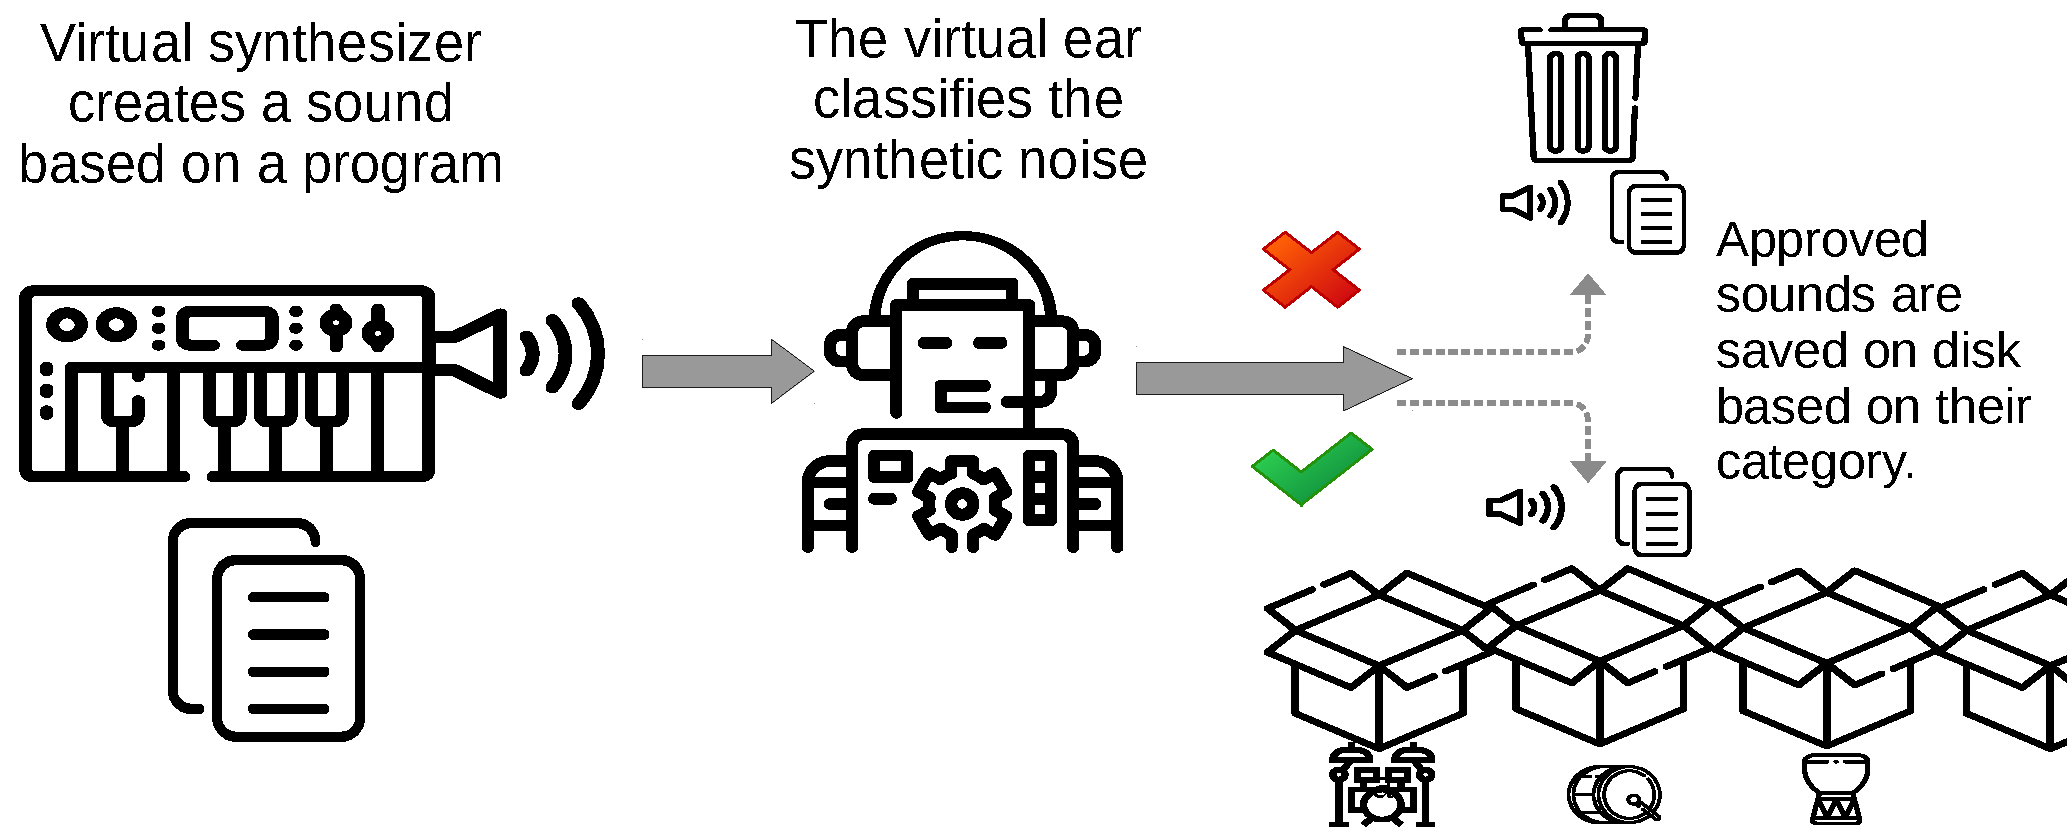
\includegraphics[width=1.1\linewidth]{images/pipeline.pdf}}}
    \end{center}
    \caption{A blueprint of our desired pipeline which allows each component to be implemented in a number of ways. Our implementations of this pipeline allow for easy parallelization when needed. 
    }
\label{fig:pipeline_outline}
\end{figure}



\subsection{Related Works}
\label{related_works}
\begin{center}
\begin{table}[h]
\resizebox{\linewidth}{!}{\begin{tabular}{|c c c c|} 
\hline
Work & Feature extraction & Synthesis & Specilization & \hline
Oord 2017 & CNN & CNN &Speech& \hline
Yee-King 2018 & LSTM on Paremters & DSP & Synth Pads & \hline
Aouameur 2019 & Latent layer& Decoding of Latent Layers & Percussion & \hline
Ramires 2020 & Latent layer & FeedForward Network & Percussion & \hline
Yamamoto 2020 & GAN & GAN & Speech & \hline
\end{tabular}}
\caption{Quick reference of recent related works}
\end{table}
\label{table:recent_works}
\end{center}
Numerous deep, neural network models have been proposed and utilized for the purpose of signal generation in recent years. WaveGans and WaveNet have been subject to significant improvements and experiments since their proposal~\cite{nsynth2017,yamamoto2020parallel,oord2017parallel}. Most relevant to us are recent works by Aoumaeur et al. in which variational AutoEncoders (VAE's) have been utilized for generation of percussive samples~\cite{aouameur2019neural}; As well as Ramires et al's work in generation of percussive sounds by guiding the output of a feedforward neural network via a small set of latent features~\cite{ramires2020neural}. 
Automatic programming of virtual synthesizers has long been a topic of interest. In early 2000s, Interactive Genetic Algorithms (IGA's) were utilized for the generation of new sounds with various sound-engines~\cite{johnson1999exploring,dahlstedt2001creating}. More recent work by Yee-King et al.~\cite{yee2018automatic} used Long short-Term Memory (LSTM) models and genetic algorithms to find the exact parameters used to create a group of sounds. The sounds approximated were made by the same virtual synthesizer, not an external source; making the eventual replication certain even with random search. Since this work appears more focused on pads and textures rather than drums, feature matching appears to not be concerned with the envelope of the sounds but rather the frequency content within arbitrary time windows. Yet another recent work by Esling et al. used a large dataset of over 10,000 presets for a commercial VST synthesizer to learn a latent parameter space which can be sampled for creation of new audio~\cite{esling2019universal}. As stated before, our work explores the rapid approximation of percussion sounds with no previous knowledge about the sonic capabilities of our virtual synthesizer, exploring the actual parameter space rather than its latent representation.

\subsection{Our Approach}
To virtually create novel drum sounds, we need a tractable, generative source of audio; One that deterministically produces audio based on a set of instructions. Additionally, we need a method of evaluation to help us determine which sounds resemble drums and are worth keeping. To enable heuristic search, we would like to know what instructions caused our audio source to make the sounds we liked. Given these two components capable of \textit{generation} and \textit{evaluation} of sounds, we build a generative pipeline of audio as depicted in figure~\ref{fig:pipeline_outline}. The success of this pipeline is dependent on the characteristics of the components responsible for the generation and evaluation of the sounds. We call these two components the \emph{virtual synthesizer} and \emph{virtual ear} respectively.  

\section{Virtual Synthesizer Design}


\begin{table}[htbp]
\centering
\resizebox{\columnwidth}{!}{\begin{tabular}{ |c|c|c| } 
\hline
Parameters & Value Range & notes and constraints\\
\hline \hline
Attack & 0-3 & A-D-S-R values relative\\
Decay & 0-3 & relative to A-S-R\\
Sustain & 0-3 & relative to A-D-R\\
Release & 0-3 & relative to A-D-S\\
OSC type & sine,square,saw & tone type\\
IsNoise & boolean & whether to \newline use OSC type to generate noise\\
Length & 0-1 second & - \\
StartTime & 0-1 second & Length+Start$<$1\\
Amplitude & 0.1-1 & 1 = max amplitude\\
Pitches(notes) & list of pitches &  range of C0(16.35hz) to B9 \\
HP filter Cuttoff & 0-20000hz & -\\
LP filter Cuttoff & 20000-HP & never lower than HP cutoff\\
Filter Order & 4,8,16 & butterworth filter order \\
\hline
\end{tabular}}
\caption{Synthesizer submodule Parameters. Despite the simplicity of the parameters and our efforts at constraining the ranges, the number of parameters that can be randomly chosen for each submodule is in the order of $10^{15}$ }
\label{table:submodule_params}
\end{table}

Sound is product of physical disturbances, causing vibrations in our mediums. Vibrations are perpetuated through air as part of an expanding, spherical front ~\cite{cook1999chap4}. A sound wave can be viewed as the result of a function which governs amplitude through time, where time and amplitude exist in continuous dimensions. Waves can be approximated via a series of samples, associating time steps to a discrete range of amplitude values.~\textit{Digital synthesis} of audio is the process of creating these discrete values.
Unlike the majority of the works mentioned in Section~\ref{related_works}, we do not employ probabilistic models for the synthesizer component. Our decision is based on the following factors:
\begin{itemize}
    \item \textit{Novelty and Creativity}: Given large sets of examples, generative models such as VAEs and GANS have proven capable of generating samples similar to the exemplars. In this work, we are not aiming for perfect imitations; Following Boden's definition of exploratory creativity as an emergent property of generative work within confined rule sets~\cite{boden2009computer}, we work within the limitations of any tractable sound source to create its  approximations of a given sound category. Within the music realm, prominent instance of exploratory creativity is the persistent aesthetics of 8-bit soundtracks, remaining popular long after the original constraints are lifted~\cite{collins2007loop}.
    \item \textit{Interpretability}: Neural networks are often described as black boxes~\cite{basheer2000artificial}. Their highly recursive structure makes modern explanation methods such as saliency maps unreliable~\cite{rudin2019stop}.  
    \item \textit{Speed of Rendering at high sampling rates}: Despite the utilization of powerful GPUs, the standard sampling rate in most audio generation work utilizing neural is under 24 khz \cite{yamamoto2020parallel,oord2017parallel,aouameur2019neural,ramires2020neural}. However, a significant number of untrained human ears can detect a change in quality of audio between sampling rates of 192 khz and the industry standard of 44.1 khz \cite{reiss2016meta}. In this work, we fix our sampling rate to the 48 khz standard. 
\end{itemize}

\begin{figure*}[htbp]
\label{fig_example_sine}
\centering
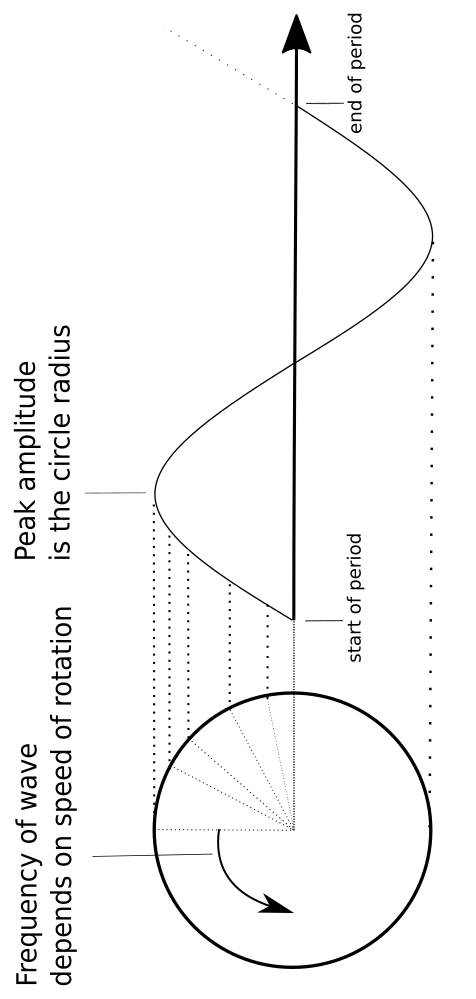
\includegraphics[width=0.45\linewidth,angle =-90 ]{images/periodic_function.png}
\caption{A computer can simulate waveforms by utilizing periodic functions. Digital waveforms are discrete approximations of analogue waves. ~\cite{mitchell2009basicsynthChap5} }
\end{figure*}

Evaluation of a periodic function such as sine or cosine is the simplest form of software audio generation~\cite{mitchell2009basicsynthChap5}. This generative system is called an \textit{oscillator}. The combination and modification of oscillators are the building blocks of digital signal processing (DSP). Most sounds from the natural environment, and its flora and fauna are more complex than the output of a single oscillator. However, with careful programming, DSP techniques can be used to replicate almost any sound, which is why they have powered commercial digital synthesizers for over half a century ~\cite{jenkins2019analog}. Another advantage to using DSP for sound generation is that the synthesizers we build using these functions are tractable: the output is determined by the input and reproducible. This makes the evaluation of a set of inputs (or parameters) to our synthesizers  simpler compared to the evaluation of synthesizers that utilize probabilistic models.
 
We opted for a set of classical DSP methods to build our synthesizer. For our project, we used the python based Pippi library for sound generation\footnote{https://github.com/luvsound/pippi}. This library uses a C back-end\footnote{https://github.com/PaulBatchelor/Soundpipe} and focuses on fast offline generation of audio signals. Our virtual synthesizer contains a set of one or more submodules. Each submodule is a self-contained noise making unit. Submodules have identical sets of parameters, but widely different outputs can be achieved depending on the values assigned. The set of parameters available to each submodule is highlighted in Table~\ref{table:submodule_params}. The sonic output of the virtual synthesizer is the normalized addition of the sonic output of its submodules. Our implementation of a synthesizer can have any number of submodules. The parameters that dictate the output signal of each submodule as well as the range of values each parameter can take are shown in table~\ref{table:submodule_params}. We call the number of submodules in each virtual synthesizer the \textit{stack size}. We call the sets of parameter values that characterize a synthesizer's submodules a \textit{program} (analogous to a preset for a VST).  

\section{Virtual Ear Design}
\subsection{Feature Extraction}
To train our virtual ear, we require the generalizable, domain agnostic features. In this work we rely entirely on Fast Fourier Transform (FFT) and by extension Short-time Fourier Transforms (STFT) for feature extraction. Using FFT, a signal can be represented by a vector with each index corresponding to a frequency-bin (a range of frequencies too close to be distinguishable) and the value at each index corresponding to the combined-magnitude of the frequencies within the bin. STFT can be employed when variations in frequency-bin intensities are of interest, often by the application of the FFT to a sliding time-window to create an estimation of frequencies present within each time-frame.

\begin{figure}[htbp]
\centering
\textbf{Visual Representation of Raw Features}\par\medskip
    \subcaptionbox{Randomly generated audio with percussive qualities, resembling a tight snare}{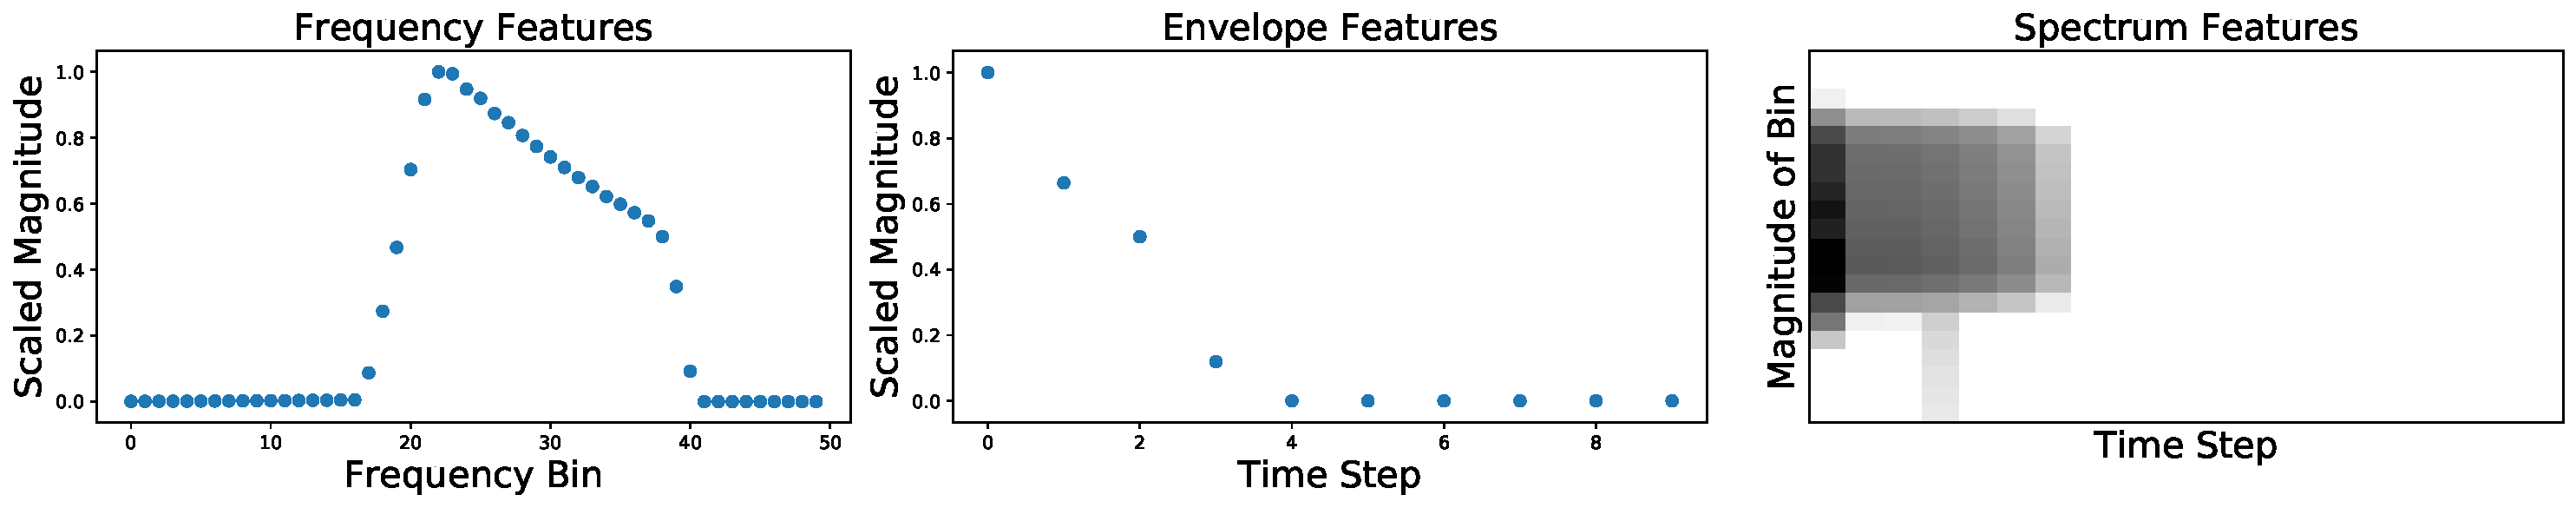
\includegraphics[width=1\columnwidth]{images/ff2.pdf}}
    \subcaptionbox{A randomly generated noise with a percussive envelop but non-percussive frequency features (modulated pitch)}
    { 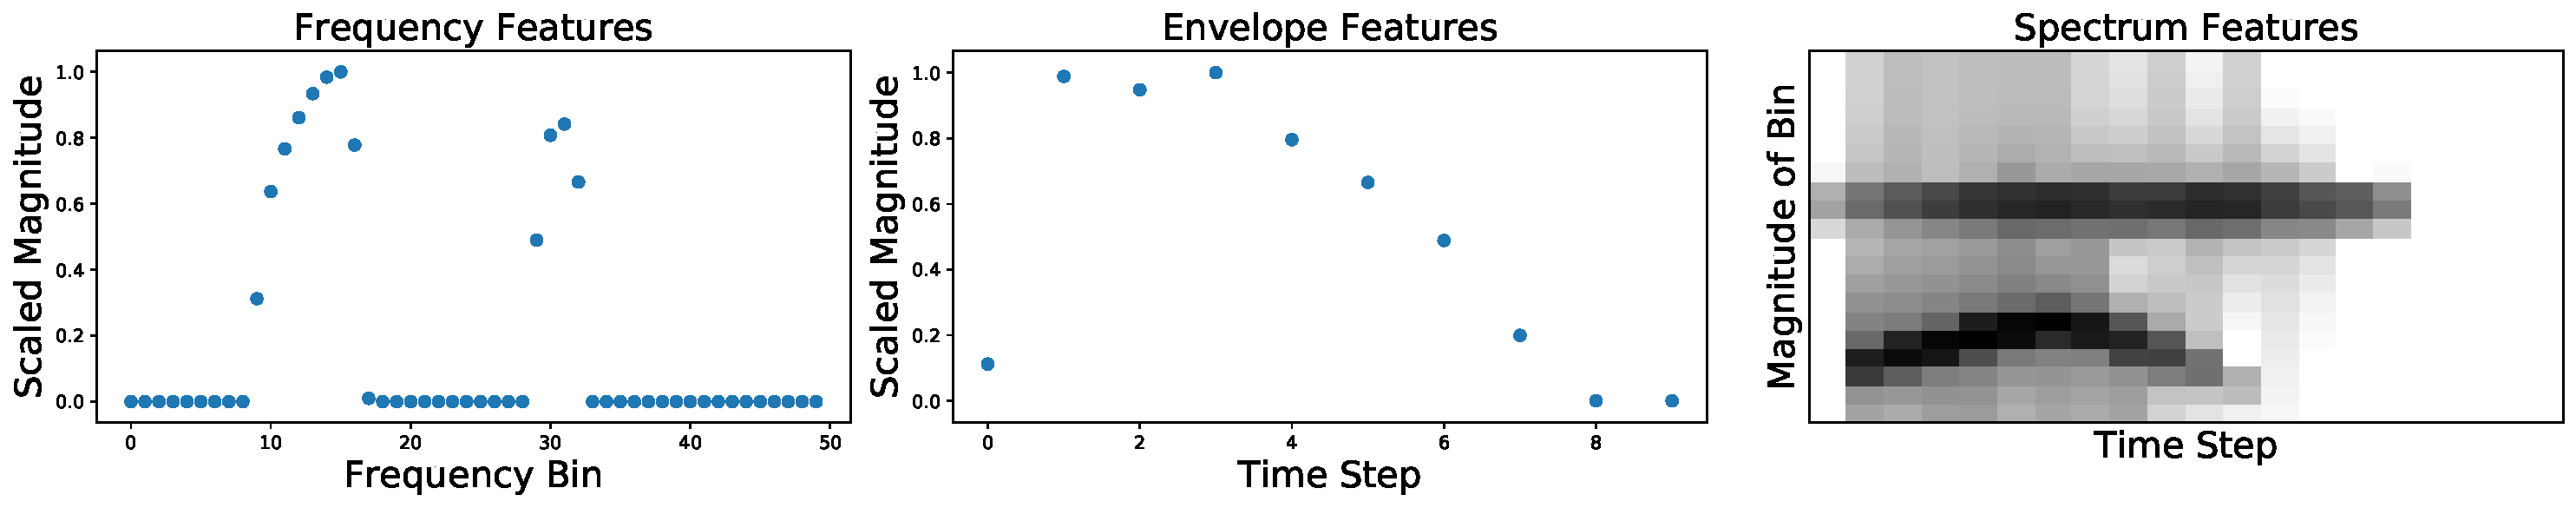
\includegraphics[width=1\columnwidth]{images/ff3.pdf}}
\caption{Graphed representation of features extracted for 2 different randomly generated samples. Sample $b$ is an example of randomly generated noise that we found suitably similar to a snare sound. Sample $c$ is an example of a randomly generated noise where the spectrum features are necessary for proper classification.}
\label{fig:stackspectrums}
\end{figure}
Various works have demonstrated effective reconstruction of signals given their STFT~\cite{nawab1983signal,griffin1984signal}. If a signal can be faithfully reconstructed from its STFT, the STFT may be relied on as source of fundamental features necessary for audible signal categorization.

Using only the STFT of signals as source of feature extraction we defined 3 transformation functions which we believe to capture important, unique attributes of percussive sounds.  These functions were applied at training time to 1 second audio samples before being sent to a classifier.


\subsection{The Models}
\label{TPE_models}
Using the described features, we trained several neural network models for Phase 1 and 2 in the Pytorch environment. The task of Phase 1 is to separate drums from not-drums (DrumVsNotDrum, or DVN). The task of Phase 2 is to categorize drums and percussion (DrumVsDrum, or DVD). We kept our feature space small, making it viable for feature selection and model design to be done on a trial and error basis. For all models, accuracy is calculated by prediction of all test dataset labels and the loss function and optimizer are Categorical-CrossEntropy and Adam respectively. Training continues until no reduction in loss and accuracy is observed in 10 epochs.  All activation functions are PReLU:
\begin {enumerate}
\item FC-DVN: Fully connected network trained on Envelope features, reaching 97\% accuracy on our test data for Phase 1. With size of 10x5x10.
\item CNNLSTM-DVN: A combination of CNN and LSTM models, where the CNN model extracts higher level features that are fed temporally to an LSTM cell. This model is trained on spectrum data and reaches 98\% accuracy on our test set. Its structure is the combination of a CNN with 2 output channels and kernel size $(7,3)$; Followed by an LSTM model of hidden size 800 and a fully connected layer of size 20x2.
\item E+F-DVD: A fully connected model trained on a concatenation of envelope and frequency features. Reaching 80\% accuracy for 6-way drum categorization in Phase 2. Size of 50x10x2x6.
\item CNN-DVD: A CNN model trained on Spectrum features. Reaching 82\% accuracy in a 6-way drum categorization in Phase 2. A combination of a CNN model with output channel size of 4, kernel of size of 5, another CNN model with output channel size of 8 and kernel of size 3. Followed by a fully connected network of shape 100x20x6.
\item FC-DVD: Fully connected 3 layer neural net with 78\% accuracy for 6-way drum categorization in Phase 2. Size of 400x200x50.
\end{enumerate}
The parameters are hand-picked and un-tuned. As discussed in Section~\ref{surveys}, higher accuracy rates in these models do not translate to higher agreeableness with humans. leading us to believe that model accuracy on test data alone cannot be relied upon when the domain of sounds 
being categorized is switched from original percussion samples to virtual synth sounds.

With our models showing high accuracy on testing data, we combine models in order to increase the efficacy of each phase and address the \enquote{open set problem} for our task. For Phase 1 we only determine sounds as percussive if both FC-DVN and CNN-LSTM have determined it as such with over 90\% confidence. For the majority of our random generations that is not the case, but if a randomly generated sound has passed this phase, our three categorizers assign their categorizations to this sound. These categorizers have a moderate degree of agree-ability as seen in~\ref{surveys}, but often the decision is not unanimous. The fourth method of categorization, \enquote{averaged-cat}, is implemented by taking the sum of the softmax outputs of all three categorizers, using it to determine the category. 

These models can be combined and weighted in various ways and the confidence thresholds can be modified in order to implement \enquote{virtual ears} with different properties. A glaring issue in the current implementation is the treatment of softmax outputs as a reasonable measure of a model's confidence. As a result, some models may have unwarranted higher confidence in their scores, skewing attempts at finding a consensus. 


\begin{enumerate}
\item Envelope Transformation: The goal of this feature is to capture the changes in loudness for the duration of the signal. Using STFT we generate a matrix $M_{i \times j}$ with rows $i$ and columns $j$ corresponding to time steps and frequency bins respectively, and with values $v_{i \times j}$ indicating the magnitude of the frequency bin $j$ at each time-step $i$. Information about the envelope of the signal can be extracted by summing the values of $M$ for each time-step (or row $i$), giving us a feature vector $v_i$. This vector is then normalized to the range of 0 to 1. The information contained in this vector is similar to that of a Root-Mean-Square measurement.
\item Frequency Transformation: A static, normalized snap-shot of the the frequencies present within the audio. The calculation of this feature vector is similar to the envelope, but the summation is done along the frequency axis. Another important distinction is that since capturing an adequate frequency resolution is important for this transformation, we utilized shorter hop-sizes and wider windows. A Mel Scale transformation was also applied in hopes that the captured features better represent human perception of frequencies. 
\item Spectrum Transformation: This function is simply a Mel Scaled STFT with its values normalized from 0-1. Since this features is a 2D matrix rather than a vector it captures more information about our signal but requires heavier, more complex computational methods to be utilized. 
\end{enumerate}


% \section{Implementation}
% We conceptualized a general pipeline for approximation of sounds: A synthesizer creates random noise while a virtual ear rapidly evaluates the outputs and outputs a score which is used for the separation of undesired outputs from desired ones. This approach assumes that a fraction of the randomly generated sounds can be substituted for percussion and that the synthetic ear will assign higher evaluation scores to this subset. 
% \begin{itemize}
%     \item \textit{Virtual Synthesizer}: A flexible, deter\-min\-istic, and tract\-able gener\-ator which can create audio. 
%     \item \textit{Virtual Ear}: An ear that returns an evaluation of an audio sample; estimating the effectiveness of an audio sample's fulfillment of a producers requirements. The ear's evaluation guides the generation process towards a desired path, making it a crucial component of our pipeline. 
% \end{itemize}



\label{gens}
\label{surveys}
\section{Results}
 In the previous chapter, we discussed our implementation of a \emph{virtual synthesizer}, which generates 1 second long sounds (or sonic noise) based on its parameters. We also discussed our expectations of an ideal \emph{virtual ear} along with multiple implementation attempts and measurements for accuracy. Putting these components together, we conceptualized a generative pipeline for creation of novel drum sounds, shown in figure~\ref{fig:pipeline_outline}.
 
 We expect the virtual synthesizer to make sounds, which we call \enquote{synthetic noise}. We also expect the ideal virtual synthesizer to create identical sounds, given the same program. We verified These claims in Section~\ref{chap3:synth_deterministic}. Much harder to verify are our expectations of the virtual ear. If a small subset of synthetic noise can stand in for percussive sounds, then the ideal synthetic ear will be able to the desired sounds from noise with high recall and precision. Low recall will cause a slow-down of the pipeline and loss of novel sounds. Low precision will make manual cleanup of generated samples a requirement. Critically, manual over-sight is necessary to assess the performance of the ear. 

To assess the performance of each pipeline, we randomly create drum programs and generate and the corresponding signal. This signal is then fed through the ear model to determine if the signal is percussive. If so, a category is assigned to the sound. This sound and the corresponding synthesizer program are saved to hard-disk. Here we assess the success rate of two different pipelines by manual inspection and categorization of a randomly selected subset of its results. We cross reference the manual categorizations with the categories assigned by the virtual ear: Do we agree that the sounds are percussive? Do we agree with the drum group assigned to the percussive sounds?
 
 \section{Survey of Two-Phased Ear Performance}
   
\begin{table}[htbp]
 \resizebox{\linewidth}{!}{\begin{tabular}{||c c c c c c c||} 
 \hline
 Drop Rule & Size & HvH & H+FC & H+CNN & H+ALL & 3 models \\ [0.5ex] 
 \hline
 No Drops & 257 &0.37 & 0.35 & 0.36 & 0.36 & 0.28\\ 
 \hline
 Assigned \enquote{Bad} By Both & 236 & 0.31 & 0.37 & 0.37 & 0.38 & 0.30 \\
 \hline
 Assigned \enquote{Bad} By Either & 180 & 0.47 & 0.50 & 0.48 & 0.48 &  0.34 \\
 \hline
 Assigned \enquote{Bad} or \enquote{Other} By Either & 154 & 0.47 & 0.59 & 0.54 & 0.50 &  0.35 \\
 \hline
\end{tabular}}
\caption{\label{kappa_table_TPE}Table of Fleiss' kappa coefficient to measure the degree of agreement between persons (HvH), persons with FC model (H+FC), persons with CNNLSTM model, persons with all models (H+ALL), and between the 3 models. \enquote{Drop Rule} column indicates if any samples were dropped. We show the measurements after dropping samples if they are deemed bad by either or both responders. We also show measurements after dropping the \enquote{other} category along with samples deemed bad by either responder. }
\end{table}
To measure the quality of the samples produced by our pipeline combined with the TP ear models, we run the model until an adequate number of samples in each category are saved to disk. Next, we randomly generated around 50 samples in the following categories: \enquote{snare}, \enquote{kick}, \enquote{hat}, \enquote{clap} and \enquote{other} (combination of rims, 
shakers and unusual percussive sounds). This gave us a total of 257 samples. These samples were determined to be percussive and then categorized by 4 different models (FC, CNNLSTM, E+F and AVG). We ensured a balanced division between samples of stack size 1, 2 and 4 (each stack is responsible for a third of the samples under each category). Both reviewers then categorized these samples without knowledge of other categorizations (person or computation models). It's important to note:
\begin{itemize}
    \item Each responder had an additional category of bad for samples that they deemed not percussive. The \enquote{bad} category indicates that the sample should have been skipped in Phase 1. 
    \item With 6 categorization groups, responders had the same categorization in 47\% of cases.
    \item The agreement between the responders and AVG was 44\% and 47\%.
    \item Of 257 samples, the responders agreed with FC, CNNLSTM, AVG and E+F respectively in 78, 76, 76 and 46 of cases. This indicates no major difference in model types and agree-ability, with E+F being the worst performer.
\end{itemize}

\begin{figure}[h!]
    \begin{center}
    \textbf{Label Assignment Frequency}
    \makebox[\textwidth]{
    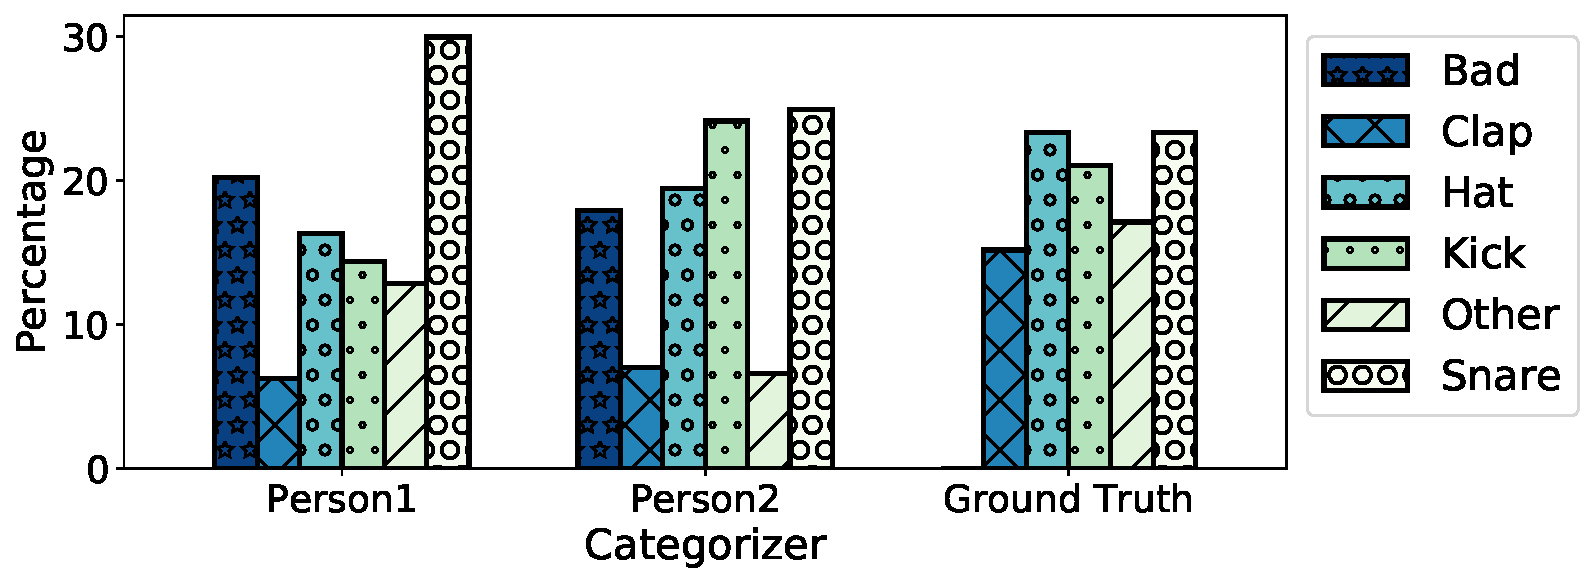
\includegraphics[width=1.1\linewidth]{images/cat_2p.pdf}}
    \end{center}
    \caption{Frequency of assigned labels by persons vs the true number of labels}
\label{fig:freq-survey-2p}
\end{figure}
We assess the reliability of agreement between persons and categorization models via the Fleiss' kappa coefficient \cite{fleiss1971measuring}. The value of 0 or less for this coefficient indicates no agreement beyond random chance, and the value of 1 indicating perfect agreement. Our kappa measurements shocased in~\ref{kappa_table_TPE} lie within the 0.35-0.45 range, indicating mild to moderate agreement between persons and machines. We again measure this coefficient after dropping samples that were categorized as \enquote{bad} by the authors, as samples that persons deem to be \enquote{bad} indicate a failure in Phase 1 and should not have been categorized by the models at all. Dropping of samples that both authors deemed \enquote{bad} causes an 8\% reduction of our data (21 samples) and a small increase in kappa score. Dropping samples deemed bad by either reviewer resulted in a 30\% reduction of samples and relatively large increase in kappa scores. 

\subsection{Takeaways Of The Two Phased Pipeline Survey}
\label{survey1_takeaway}
\begin{itemize}
    \item The survey brings into question the reliability of our phase 1 models, as 30\% of the generated samples were deemed not percussive by at least 1 reviewer and 8\% by both reviewers
    \item The task of categorizing synthetic drums is difficult. Survey shows that the scale of agreement within persons as well as between persons and various model combinations is moderate at best, even after removal of \enquote{bad} samples.  While the same models can easily achieve 98+ percent accuracy when tested on recorded drum samples. This may be a manifestation of the \enquote{open set recognition} problem. 
    \item While there is much room for improvement, our pipeline can generate and categorize drums and percussive sounds with a promising degree of success. 
\end{itemize}

 \section{Survey of Mixed-Models Ear Performance}
 Keeping the other components of the pipeline the same, we replace the two-phased ear in the previous pipeline with the MME. Our survey differs from the previous survey in that the pipeline only creates the four drum categories. The \enquote{other} category is only assigned by survey responders. This means that two out of six possible categories are only available to responders, therefore there is an inherent bias towards worse agreeably scores compared to last survey. Our main concern here is changes in the amount of \enquote{bad} samples. We show measurments before and after dropping all \enquote{bad} and \enquote{other} samples for a fairer comparison with the TPE pipeline.

 \begin{table}[t]
 \resizebox{\linewidth}{!}{\begin{tabular}{||c c c c||} 
 \hline
 Drop Rule & Size & HvH & H+MME \\
 \hline
 No Drop & 300 & 0.336 & 0.250\\ 
 \hline
 Assigned Bad By Both & 249 & 0.200 & 0.260 \\
 \hline
 Assigned Bad By Either & 151 & 0.460 &  0.473 \\
 \hline
Assigned \enquote{Bad} or \enquote{Other} By Either  & 120 & 0.620   &  0.587 \\
 \hline
\end{tabular}}
\caption{\label{kappa_table_MME}Table of Fleiss' kappa coefficient to measure the degree of agreement between persons (HvH) and persons and MME. We also measure the agreeability scores after dropping bad samples if both or either persons assigned the sample as such. We also measure agree-ability when all samples deemed \enquote{bad} or \enquote{other} by either person are removed.}
\end{table}

\begin{figure}[htpb]
    \begin{center}
    \textbf{Category Assignment Frequency For MME Survey}
    \makebox[\textwidth]{
    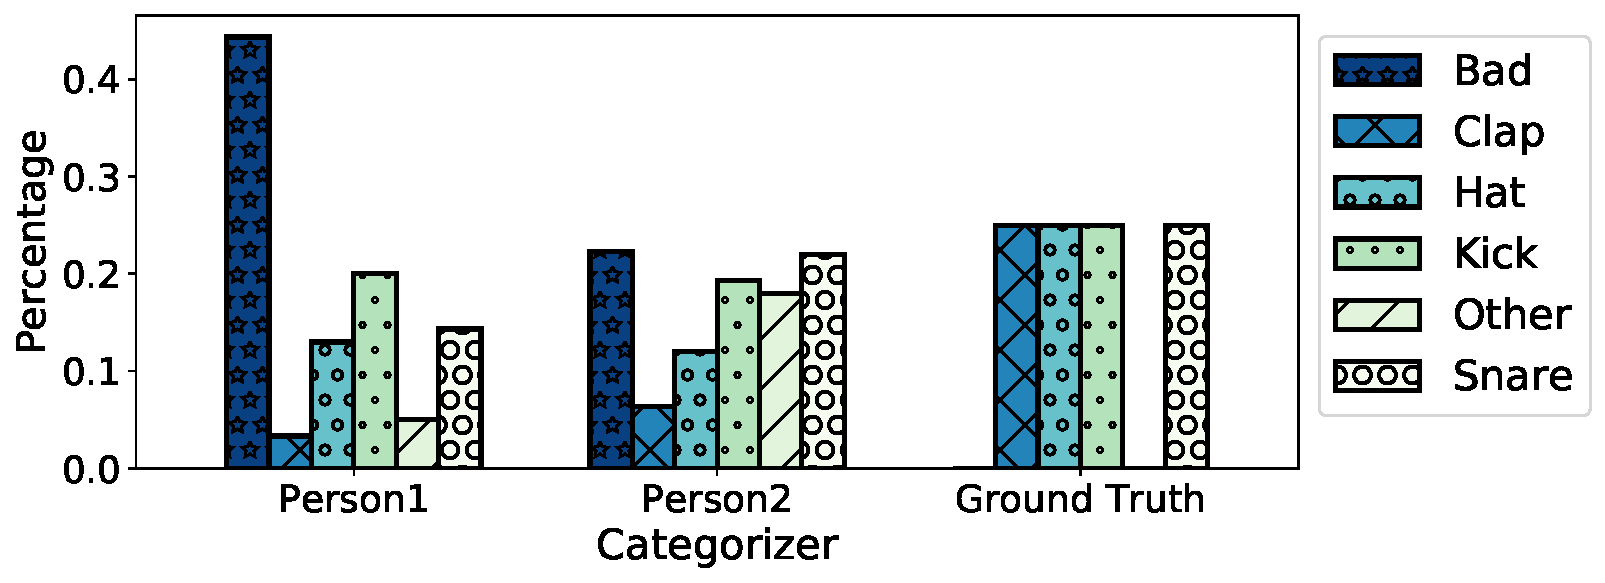
\includegraphics[width=1.1\linewidth]{images/cat_mme.pdf}}
    \end{center}
    \caption{Frequency of assigned labels by persons vs the true number of labels}
\label{fig:freq-survey-2p}
\end{figure} 
\subsection{Takeaways Of The MME Pipeline Survey}
\label{survey2_takeaway}
The results from the two surveys are not easily comparable. However, no major improvements in agree-ability or a decrease in the number of bad samples can be seen, in fact, the opposite is more likely to be true. However, we are yielding comparable results to the TPE pipeline despite having a fraction of the features to learn from (latent layer + 10 envelope features). This shows that latent layers of an autoencoder network can be used as a low-dimensional proxy for representation of more complex inputs, despite the autoencoder not being trained for such a task. 

Agree-ability scores for MME pipeline are often lower, but we reiterate that this can be caused by having two out of six (rather than one out of six in the TPE pipeline) categories which are exclusive to survey responders. Supporting this hypothesis is the notable improvement in agree-ability observed after dropping all \enquote{bad} and \enquote{other} samples. Here, both persons agree with each other and with the MME at a stronger rate than in the TPE pipeline, despite having similar number of samples (120 for MME and 154 for TPE) and equal number of categories to choose from. This values are observed in the last rows of tables~\ref{kappa_table_TPE} and ~\ref{kappa_table_MME}. The higher DVD categorization accuracy achieved by the mixed-model ear compared to the best two-phaased ear is consistent with this observation: Given that the sound being categorized is a drum, the MME will yield better results that the TPE. However, the MME pipeline does not yield better results in the DVN task. 
\bibliographystyle{apacite}
\bibliography{CSMC_MUME_LaTeX_Template.bib}

\begin{appendices}
\chapter{Datasets}
\begin{table}[h!]
\centering
\begin{tabular}[width=\paperwidth]{|l|l|l|l|l|l|l|l|l|l|}
\hline
DB Name & kick & snare & clap & tom\_high & tom\_mid & tom\_low & hihat\_closed &  hihat\_open & rim \\ \hline
MixedDB & 648 & 732 & 118 & 179 & 139 &  188 & 187 & 280 & 105 \\\hline
\end{tabular}
\caption{Database 1: Mixed sources}
\label{db:self}
\end{table}

\begin{table}[h!]
\centering
\begin{tabular}{|l|l|l|l|l|l|l|l|l|}
\hline
DB Name & kick & snare & clap & tom & clap & hat & rim & shaker  \\ \hline
RadarDB & 1054 & 842   & 353 & 349 &  353 & 1561& 131 & 121 \\ \hline
\end{tabular}
\caption{Database 2: Royalty free sounds sourced from \enquote{Music Radar}}
\label{db:radar}
\end{table}

\begin{table}[h!]
\centering
\begin{tabular}{|l|l|l|l|l|l|}
\hline
 DB Name & kick & snare & clap & hat & other \\\hline
 FreeDB & 533 & 372 & 230 & 105 & 281 \\ \hline
\end{tabular}
\caption{Database 3: Free sounds sourced from the \enquote{Sample Swap} project. Simplified for our purposes. The version available for download contains more sample groups. The \enquote{other} category contains a variety of percussive sounds.}
\label{db:sampleswap}
\end{table}


\begin{table}[h!]
\centering
\begin{tabular}{|l|l|l|l|}
\hline
 Synth Noise Type & 1 Stack & 3 Stacks  & 5 Stacks \\ \hline
 Number of Examples & 2000 & 2000 & 2000 \\ \hline
\end{tabular}
\caption{Database of random noise examples from our virtual synthesizers}
\label{db:noise}
\end{table}

\chapter{Virtual Ear Models}
% \begin{table}[htbp]
% \centering
% \begin{tabular}{|p{3cm}|p{8cm}|}
% \hline
%  Merged Name & Possible Merged Groups \\ \hline
%  Kicks & low toms and kicks \\
%  Toms & toms and mid toms \\
%  Snares & snares and high toms  \\
%  Hats & high hats and low hats \\ 
%  Other & rims, shakers and other percussive sounds with few representative samples \\ \hline
% \end{tabular}
% \caption{These mappings may be used to simplify databases. }
% \label{db:merge-map}
% \end{table}
\end{appendices}


\end{document}
